\documentclass{ctexart}

\usepackage{graphicx}
\graphicspath{{figures/}}

%figure环境(table环境类似)
%\begin{figure}[允许位置]
%	<任意内容>
%\end{figure}
%
%允许位置参数(默认tbp)
%h为此处(here)-代码所在的上下文位置
%t为页顶(top)-代码所在页面或之后页面的顶部
%b为页底(bottom)-代码所在页面或之后页面的底部
%p为独立一页(page)-浮动页面

\begin{document}
	\LaTeX{}中的插图见图\ref{poca}。	%引用标签
	\begin{figure}[htbp]	%figure浮动体环境
		\centering	%使环境中内容居中排版
		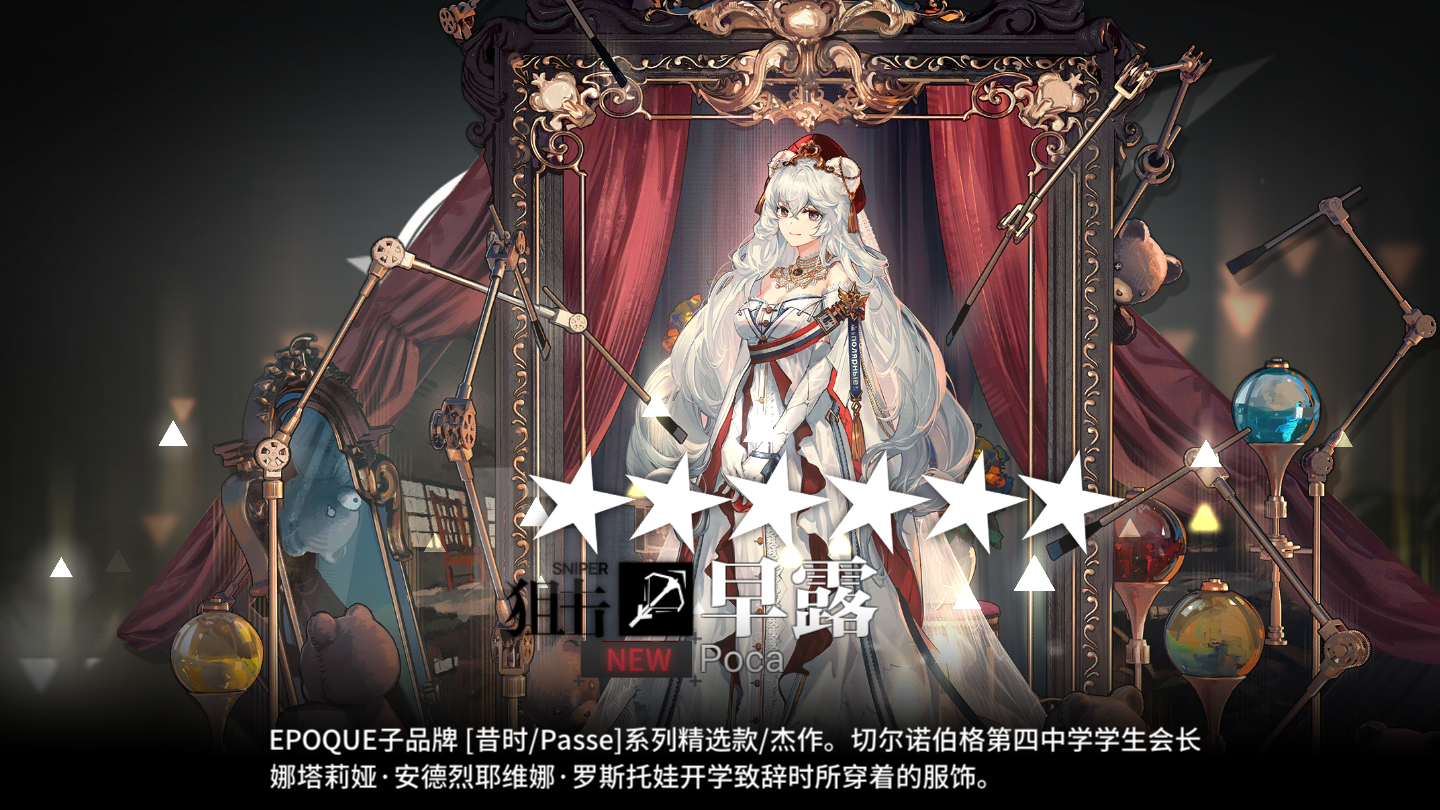
\includegraphics[scale=0.5,width=0.7\textwidth]{Poca}
		\caption{早露—杰作}\label{poca}	%设置标题、标签
	\end{figure}

	
	\LaTeX{}中的表格:
	\begin{table}[h]	%table浮动体环境
		\centering	%使环境中内容居中排版
		\caption{考试成绩单}
		\begin{tabular}{l || c | c | c | p{1.5cm}}	
		\hline	%产生表格横线
		姓名 & 语文 & 数学 & 外语 & 备注 \\
		\hline \hline
		张三 & 87	& 100 & 93 & 优秀 \\
		\hline
		李四 & 75 & 64 & 52 & 补考另行通知 \\
		\hline
		王二 & 80 & 82 & 78 & \\
		\hline
		\end{tabular}
	\end{table}

\end{document}